\subsection{Double DQN}
Q-learning  and DQN tend to learn overestimated action values. During the maximization over the action choices, values are rather over than underestimated.
This isn't necessarily a problem if they are uniformly overestimated or if interesting experiences are overestimated. However, in DQN overestimations differ for different actions and states. Combined with bootstrapping, this results in the propagation of wrong values and thus to worse policies \cite{DBLP:journals/corr/HasseltGS15}. To reduce those overestimations, the Double Q-learning algorithm \cite{DBLP:journals/corr/HasseltGS15} is used. 
The main idea of the Double Q-learning algorithm is to decouple value selection and evaluation.
DQN, with separate online and target networks provides an excellent framework for this decoupling:
The online network is used to select an action from the action choices via maximization whereas the target network evaluates the actions to generate the Q-values.
The resulting double DQN yields more accurate values and hence leads to better policies than DQN \cite{DBLP:journals/corr/HasseltGS15}.
Updating double DQNs is similar to updating DQNs when the target is rewritten as:
\begin{equation}\label{eq:DDQN-target}
Y_{t}^{\text { Double DQN }} \equiv R_{t+1}+\gamma Q\left(s_{t+1}, \underset{a}{\operatorname{argmax}} Q\left(s_{t+1}, a ; \theta_{t}\right); \theta_{t}^{-}\right).
\end{equation}
$\theta_{t}^{-}$ and $\theta_{t}$ are the weights of the target and online network respectively.
\subsection{Prioritized Experience Replay}
In standard experience replay, the agent is forced to pick experiences uniformly from all experiences in its memory. Therefore all experiences are sampled with the same frequency that they were originally encountered.
This is not necessarily good for the learning process, as some experiences might not hold any valuable information for the agent but occur very often while other rare situations could be crucial for learning. \\
This can be improved by prioritized experience replay \cite{DBLP:journals/corr/SchaulQAS15}. Here every experience in the buffer gets a priority according to its TD-error.
The TD-error measures the difference between the actual Q-value and the Target-Q-value, so if experiences with bigger TD-errors are provided with bigger priorities, experiences from which there still is a lot to learn are favoured.
The priority $p_i$ is determined from the TD-error $\delta_i$ according to:
\begin{equation}
p_{i}=\left|\delta_{i}\right|+\epsilon.
\end{equation}
Hereby $\epsilon\,>\,0$ denotes a small parameter to ensure, that every experience has a priority bigger than zero and thus can be picked for a sample batch.
New experiences are always added with maximum priority to the memory.
Problematic with this greedy approach is, that only experiences that are picked for learning get their priority updated. Therefore experiences with low initial priority might, because of the buffer memory structure be removed from memory before they could have been picked for learning. The buffer is also very sensitive to noise spikes \cite{DBLP:journals/corr/SchaulQAS15}. \\
To overcome this problems stochastic prioritization is used and $p_i$ adjusted according to:
\begin{equation}
P(i)=\frac{p_{i}^{\alpha}}{\sum_{k} p_{k}^{\alpha}}.
\end{equation}
Here $\alpha\,\epsilon\,[0,1]$ is another parameter which adjusts the amount of prioritization that is used. For $\alpha=0$ we get the uniform case (no prioritization), whereas $\alpha=1$ leads to greedy prioritization. \\
Stochastic prioritization introduces bias to our model. This needs to be considered for updating the model, because it could change the solution the model is converging to \cite{DBLP:journals/corr/SchaulQAS15}. To correct this, importance sampling weights (IS weights) are introduced: 
\begin{equation}
w_{i}=\left(\frac{1}{N} \cdot \frac{1}{P(i)}\right)^{\beta},
\end{equation}
with N being the replay buffer size and $\beta\,\epsilon\,[0,1]$ being a hyperparameter for  adjustment of the bias. 
For $\beta=1$ the bias gets fully compensated. This is most important at the end of the training process. Therefore $\beta$ starts at an initial value and is then being annealed during training. \\\\
An efficient data structure for the memory is crucial for good performance.
To guarantee this, we implemented a sum tree to store the data, where searching is of complexity $O(1)$ and updating of complexity $O(\log N)$.
A sum tree is a binary tree, in which the parent node values are the sum of the child node values. In our sum tree, the transition priorities were saved in the leave nodes. Therefore the root holds the total priority. An array was used to hold the associated data values to the priorities. For the purpose of sampling the total priority is divided into k priority ranges, with k being the number of experiences in one sample.
From each of these priority ranges one value is sampled uniformly and its corresponding leave node is searched. The data belonging to this priority is than used for the sample.

\subsection{Duelling networks}
The idea behind duelling networks \cite{DBLP:journals/corr/WangFL15} is, that for some states only the state-value function is important while for others the chosen action is crucial. \\
Consider a small toy problem: Our agent needs to catch coins which are falling down form above, he can either move right or left or wait to catch them. In some states there are no coins at all. In that state it is not important which action is chosen, whereas for other states its is.
\begin{figure}
\centering
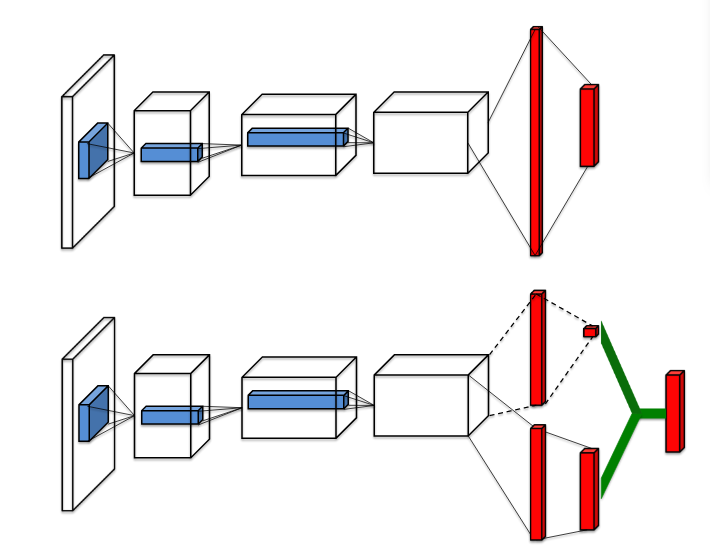
\includegraphics[scale=0.5]{./images/dueling.png}
\caption{Top: Standard Deep Q-network. Bottom: Dueling DQN with two separate streams \cite{DBLP:journals/corr/WangFL15}.}
\label{fig: dueling}
\end{figure}
To exploit this the neural network is split into two streams: 
the action and the state-value stream, as can be seen in figure \ref{fig: dueling}. The network is split after the convolutional layers. Therefore the two streams consist of linear layers. The benefit of this is, that it is possible to get separate estimations for state-value function and action-value function. Hereby the state-value $V(s ; \theta, \beta)$ is a scalar property while the action-vector $A(s, a ; \theta, \alpha)$ has the dimension of the quantity of possible action choices, in our case six. $\theta$ are the weights of the convolutional layers, while $\alpha$ and $\beta$ are the weights for the A- and the V- stream respectively. \\
For getting the Q-value A and V need to be recombined. It is not a good idea though to simply add them together:
\begin{equation}
Q(s, a ; \theta, \alpha, \beta)=V(s ; \theta, \beta)+A(s, a ; \theta, \alpha).
\end{equation}
In that case it would get impossible to retrieve V and A from Q uniquely. One could add a constant to A and subtract it from V without changing Q.
It is better to calculate Q by
\begin{equation}
Q(s, a ; \theta, \alpha, \beta)=V(s ; \theta, \beta)+ \left(A(s, a ; \theta, \alpha)-\frac{1}{|\mathcal{A}|} \sum_{a^{\prime}} A\left(s, a^{\prime} ; \theta, \alpha\right)\right),
\end{equation}
where A and V keep their identifiability and the optimization becomes more stable \cite{DBLP:journals/corr/WangFL15}.
\subsection{Noisy Networks}
So far we did use an $\epsilon$-greedy policy for exploration. Another technique which has been found to produce better result for many of the Atari games are Noisy Nets \cite{DBLP:journals/corr/FortunatoAPMOGM17}. They add parametric noise to the weights and thus aid exploration without the need to pick random actions as part of a policy (e.g. $\epsilon$-greedy). This is very convenient, because there is no need to tune additional hyper parameters as the reinforcement learning algorithm tunes the weights automatically.
Consider a neural network $y=f_{\theta_n}(x)$. Where $\theta_n$ are the noisy weights. A linear layer of a neural network can be written as: 
\begin{equation}
y = w x+b,
\end{equation}
whereas a noisy linear layer can be written as:
\begin{equation}
y =\left(\mu^{w}+\sigma^{w} \odot \varepsilon^{w}\right) x+\mu^{b}+\sigma^{b} \odot \varepsilon^{b}.
\end{equation}
Here $x$ is the input, $w$, and $\mu^{w}+\sigma^{w} \odot \varepsilon^{w}$ are the weights and $b$ and $\mu^{b}+\sigma^{b} \odot \varepsilon^{b}$ are the biases for linear and noisy linear layer respectively. All of the named parameters are trainable except for $\varepsilon^w$ and $\varepsilon^b$ which are noise random variables. We chose factorized gaussian noise for the distribution of the $\varepsilon$ parameters, as it reduces computation time for random number generation, which is important for single thread-agents such as ours \cite{DBLP:journals/corr/FortunatoAPMOGM17}. Here only one independent noise per input and another independent noise per output is needed, in contrast to independent Gaussian noise, where one independent noise per weight would be required.
We factorized $\varepsilon^w$ to $\varepsilon^w_{i,j}$.
The noise random variables can then be written as:
\begin{equation}
\begin{aligned} \varepsilon_{i, j}^{w} &=f\left(\varepsilon_{i}\right) f\left(\varepsilon_{j}\right) \\ \varepsilon_{j}^{b} &=f\left(\varepsilon_{j}\right) \end{aligned},
\end{equation}
where we used \begin{equation}
f(x)=\operatorname{sgn}(x) \sqrt{|x|}.
\end{equation}
The parameters $\mu_{i,j}$ were initialized as samples from a random uniform distribution $\left[-\frac{1}{\sqrt{p}},+\frac{1}{\sqrt{p}}\right]$ with $p$ being the number of inputs for the noisy linear layer. $\sigma_{i, j}$ were set as $\sigma_{i, j}=\frac{\sigma_{0}}{\sqrt{p}}$. \\
For the Noisy Networks implementation we replaced the Fully Dense layers of the state-value and action streams by Noisy layers. %TODO Loss changes?
\cite{DBLP:journals/corr/FortunatoAPMOGM17}